%! Author = sbbfti
%! Date = 10/06/2020


\section{Results}\label{sec:results}

The sensible heat losses from the skin to the environment are proportional to the difference between the \ac{t-sk} and \ac{t-op}.
Consequently for values of \ac{t-op} higher than \ac{t-sk} the term \ac{c-r} becomes negative, or in other words the body gains sensible heat from its environment.
Figure~\ref{fig:comparison_models}A shows how the sensible heat losses estimated with the \mycite{GaggeSET} and the \mycite{Jay2015} models vary as a function of the \ac{t-op}, \ac{rh}, and \ac{v}.
While the \mycite{Jay2015} models assumes the \ac{t-sk} to be constant and equal to 35~°C \mycite{GaggeSET} models iteratively determine skin temperature.
This explains the difference in \ac{c-r} determined by the two models.
For \ac{t-op} higher than those at which \ac{w-max} occurs, \ac{t-sk} increases and consequently the sensible heat gains do not increase as much as estimated by \mycite{Jay2015}.
The values of \ac{w} and the respective values of \ac{w-max} for two air speeds are shown in Figure~\ref{fig:comparison_models}B.

The negative effect that \ac{v} has on the sensible heat losses is, however, compensated by a larger increase in the value of \ac{e-max}.
Figure~\ref{fig:comparison_models}D shows the values of \ac{e-max} estimated by replacing \ac{w} in Eq.~\ref{eq:latent-skin} with \ac{w-max}.

It can be observed that for a fixed increase in \ac{v}, the relative increase in \ac{e-max} decreases as the \ac{rh} increase.
Finally, Figure~\ref{fig:comparison_models}C shows the estimated \ac{m-sweat}.
While, \mycite{Jay2015} does not set an upper limit for \ac{m-sweat}, \mycite{GaggeSET} imposes that the maximum value of \ac{m-sweat} cannot exceed 500 mL/h. % todo check units
In addition, it can be observed that the sweating rate estimated by the two models significantly differs.
% todo describe discrepancies

\begin{figure}
    \centering
    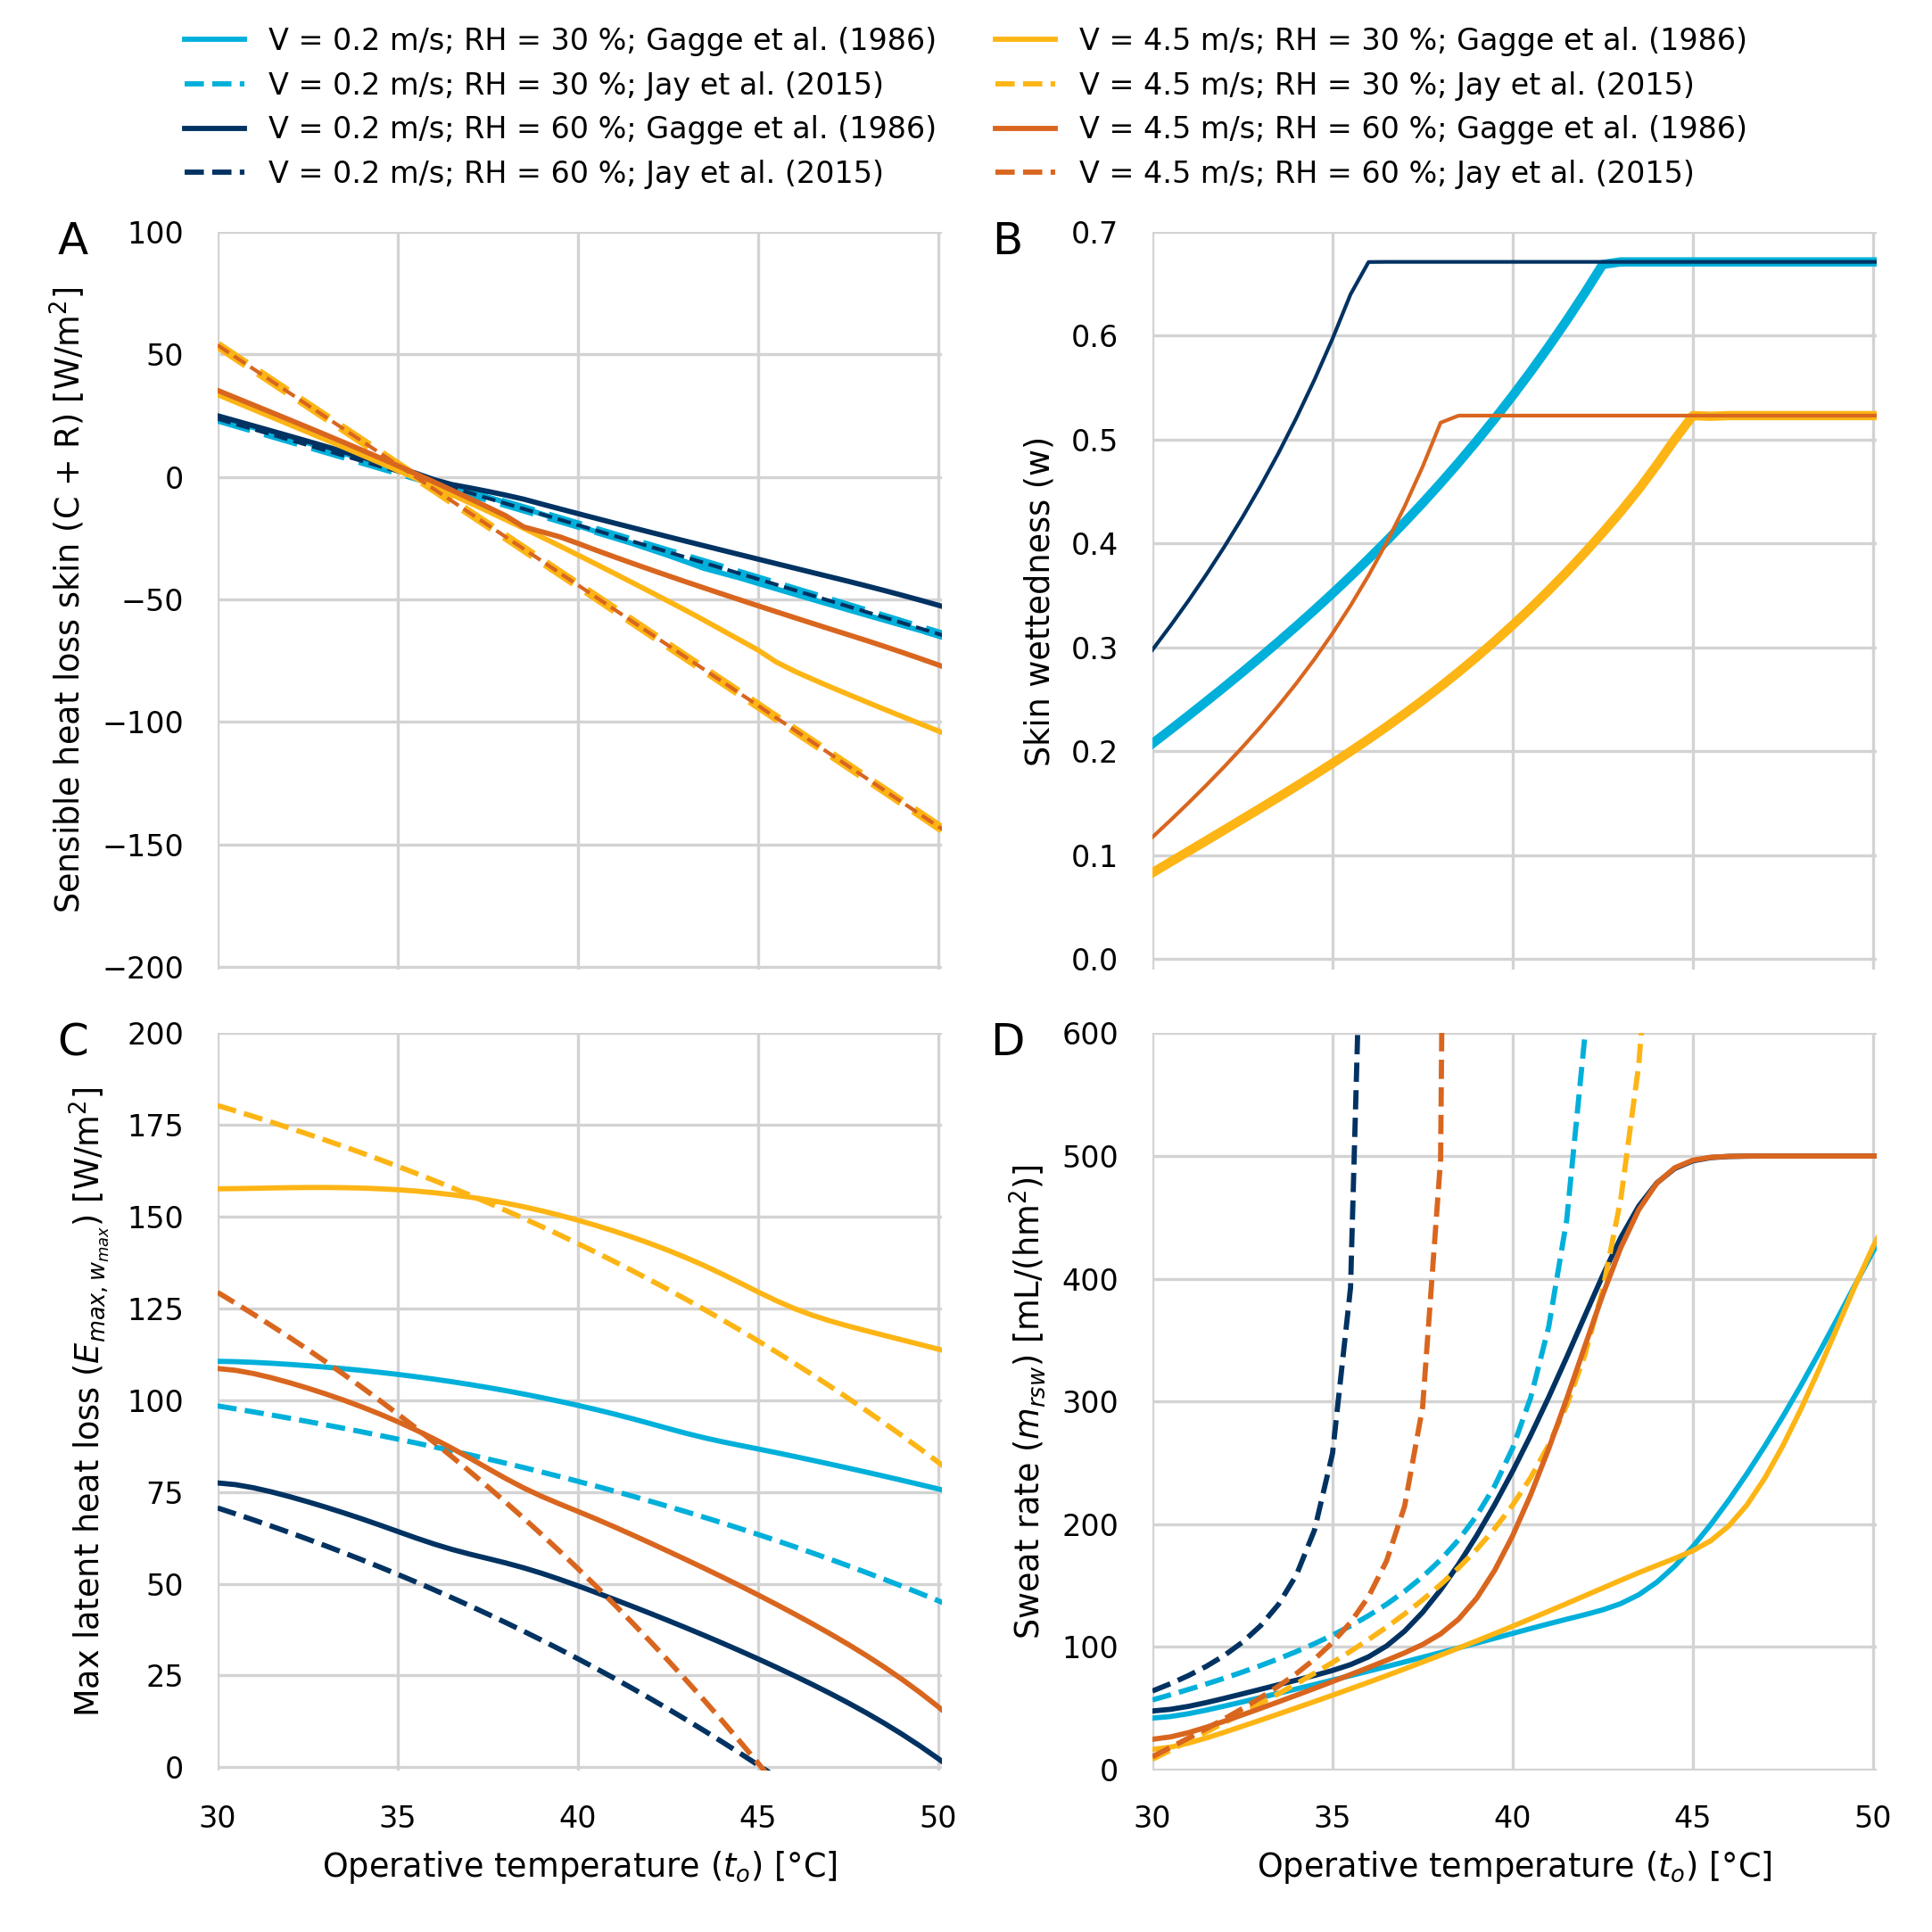
\includegraphics[width=\textwidth]{figures/comparison_models_v2.png}
    \caption{Shows how the results obtained with the the energy models proposed by \mycite{Jay2015} and \mycite{GaggeSET} vary as a function of the \ac{t-op}.
    Each Figure shows the results obtained using a combination of two values of \ac{rh} and \ac{v}.
    Figure A - sensible heat losses from the skin vary.
    Figure B - skin wettendess.
    Figure C - Maximum latent heat loss estimated using \ac{w} = \ac{w-max}.
    Figure D - Sweat rate.}
    \label{fig:comparison_models}
\end{figure}

The \mycite{GaggeSET} model was then used to determine at which combination of \ac{t-op}, \ac{rh}, and \ac{v} \ac{w} would exceed \ac{w-max}, hence the maximum skin wettedness would not longer increase, results are presented in Figure~\ref{fig:comparison_air_speed}.
The Figure shows both the results obtained with the\mycite{GaggeSET} and the \mycite{Jay2015} models.
It should, however, be noted that the limit presented in Figure~\ref{fig:comparison_air_speed} is not the limit above which an increase in \ac{v} is no longer beneficial and would lead to higher thermal loads to the human body than the still air scenario.
The limit only demarcates the region in which thermal stress is estimated to occur.
The environmental conditions above which the use of elevated air speeds would actually be detrimental for the health of the people is shown in Figure~\ref{fig:energy_storage_delta}.
This figure depicts the environmental conditions above which the heat balance model would estimate that the \ac{t-cr} would be higher with \ac{v} of XX~m/s rather than with 0.1~m/s.
This would occur since the sensible heat gains caused by forced convection, would exceed the heat losses from the body towards its surrounding environment.

% todo report estimated sweat heat lossess too, either using a table or a heatmap


%\begin{itemize}
%    \item I do not really see the benefit of the model proposed by Hosper since: 1) they set the limit of sweating to 440 mL/h; and they limit 2) the amount of water than I person can spray on him self to 116 mL/h. This would not affect the results in the SET model since with the SET model the estimated sweating rate is lower.
%    On the other hand it affects the result in the Ollie model since the exponential growth of the sweat rate in their model is more marked.
%    Moreover, very dry climates could benefit from using evaporative cooling.
%\end{itemize}

\begin{figure}
    \centering
    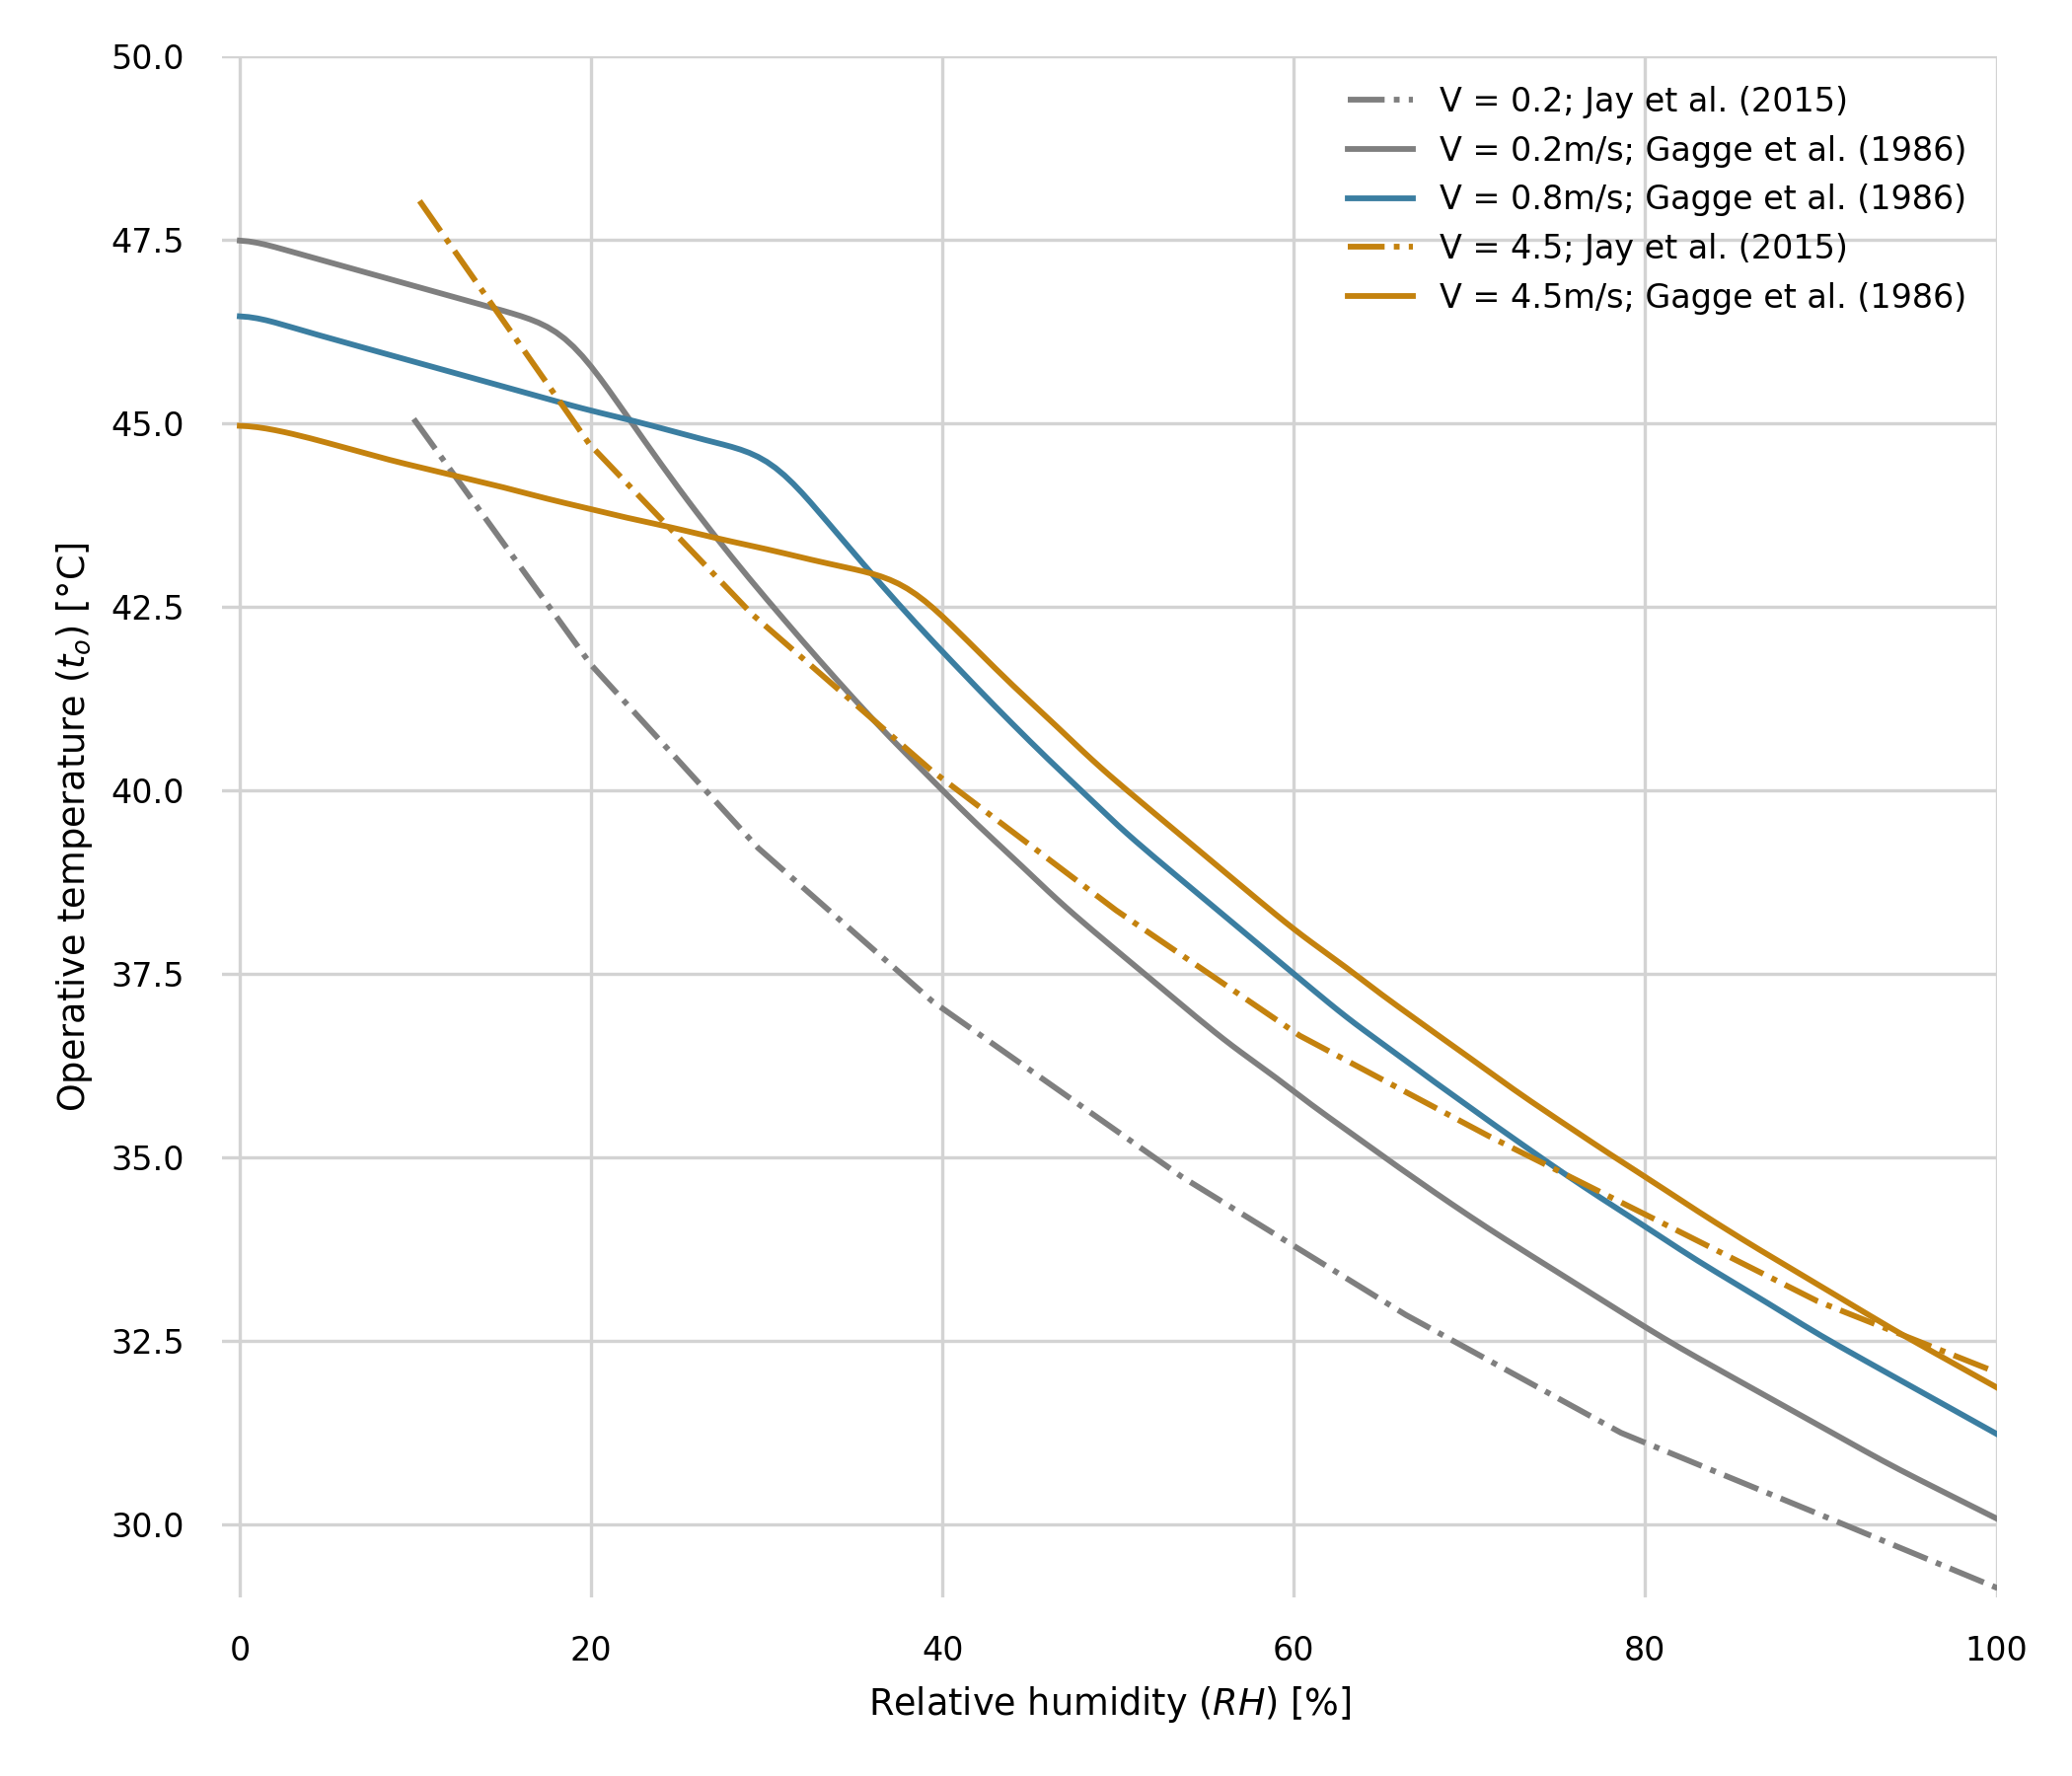
\includegraphics[width=\textwidth]{figures/comparison_air_speed.png}
    \caption{Compares the results between the SET model and Ollie's model.
    Each line demarcates the boundary between acceptable cardiovascular strain (below line) and elevated cardiovascular strain (above the line).
    Above the line the latent heat that needs to be dissipated exceeds the amount of latent heat that the same individual can dissipate. }
    \label{fig:comparison_air_speed}
    % todo extend the lines to the top left border, add units to axis and change label to opertative temperature
\end{figure}

For a set value of \ac{v}, the maximum \ac{t-op} at which cardiovascular strain is estimated to occur by the model decreases as the value of \ac{rh} increases.
In addition, it can be observed that for a specific value of \ac{rh}, as the value of \ac{v} increases the overall increase in the maximum critical temperature rapidly decreases.
Consequently, for example in an environment at 60~\% \ac{rh}, increasing \ac{v} from 0.1~m/s to 0.8~m/s then to 4.5~m/s lead to an increase of the critical temperature of approximately 2~°C and 0.5~°C, respectively.

\begin{figure}
    \centering
    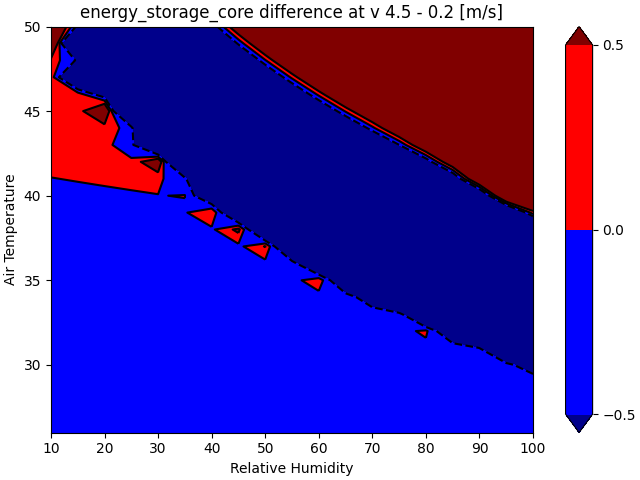
\includegraphics[width=\textwidth]{figures/energy_storage_delta.png}
    \caption{Caption}
    \label{fig:energy_storage_delta}
%    todo replace this figure with the core body delta
\end{figure}


